\documentclass{article}

% content/resources/templates/preamble.tex
\usepackage[margin=0.6in]{geometry}
\author{Milav Dabgar}
\usepackage{amsmath,amssymb,amsthm}
\usepackage{booktabs}
\usepackage{multirow}
\usepackage{xcolor}
\usepackage{tcolorbox}
\tcbuselibrary{breakable,skins}
\usepackage[colorlinks=true,linkcolor=blue]{hyperref}
\usepackage{titlesec}
\usepackage{enumitem}
\usepackage{tikz}
\usepackage{pgfplots}
\usepackage{circuitikz}
\usepackage[version=4]{mhchem}
\usepackage{longtable}
\usepackage{array}
\usepackage{float}
\usepackage{caption}
\usepackage{listings}

\lstset{
  basicstyle=\small\ttfamily,
  breaklines=true,
  breakatwhitespace=false,
  postbreak=\mbox{\textcolor{red}{$\hookrightarrow$}\space},
  float=false,
  numbers=left,
  numberstyle=\tiny\color{gray},
  numbersep=10pt,
  xleftmargin=2em,
  keywordstyle=\color{blue},
  commentstyle=\color{green!60!black},
  stringstyle=\color{purple},
  backgroundcolor=\color{gray!5},
  showstringspaces=false,
  tabsize=2,
  captionpos=b,
  keepspaces=true,
  columns=flexible
}

\pgfplotsset{compat=1.18}
\usetikzlibrary{shapes,arrows,positioning,calc,patterns,decorations.pathmorphing,decorations.markings,arrows.meta}

% Color scheme
\definecolor{headcolor}{RGB}{0,102,204}
\definecolor{keycolor}{RGB}{220,20,60}
\definecolor{solutioncolor}{RGB}{34,139,34}
\definecolor{mnemoniccolor}{RGB}{148,0,211}
\definecolor{codecolor}{RGB}{0,0,100}

% Spacing
\setlength{\parskip}{3pt}
\setlist[itemize]{nosep}
\setlist[enumerate]{nosep}

% Title formatting
\titleformat{\section}{\Large\bfseries\color{headcolor}}{\thesection}{1em}{}
\titleformat{\subsection}{\large\bfseries\color{headcolor}}{\thesubsection}{1em}{}

% Pandoc tightlist compatibility
\providecommand{\tightlist}{%
  \setlength{\itemsep}{0pt}\setlength{\parskip}{0pt}}

% Pandoc longtable compatibility
\newcounter{none}
\def\thenone{}


% content/resources/templates/english-boxes.tex

% Custom environments
\newtcolorbox{solutionbox}{
 breakable,
 enhanced,
 colback=solutioncolor!5!white,
 colframe=solutioncolor!75!black,
 fonttitle=\bfseries,
 title=Solution
}

\newtcolorbox{solutionboxnobreak}{
 colback=solutioncolor!5!white,
 colframe=solutioncolor!75!black,
 fonttitle=\bfseries,
 title=Solution
}

\newtcolorbox{keyformula}{
 breakable,
 enhanced,
 colback=keycolor!5!white,
 colframe=keycolor!75!black,
 fonttitle=\bfseries,
 title=Key Formula
}

\newtcolorbox{mnemonicboxenv}{
 breakable,
 enhanced,
 colback=mnemoniccolor!5!white,
 colframe=mnemoniccolor!75!black,
 fonttitle=\bfseries,
 title=Mnemonic
}

\newcommand{\mnemonicbox}[1]{%
  \begin{mnemonicboxenv}
    #1
  \end{mnemonicboxenv}
}


% Custom commands for GTU solutions
% This file defines semantic commands for consistent formatting

% Question command with automatic formatting
\newcommand{\question}[2]{%
  \section*{Question #1}%
  \textbf{#2}%
}

% OR question variant
\newcommand{\questionor}[2]{%
  \section*{Question #1 OR}%
  \textbf{#2}%
}

% Proper table environment with caption
\newenvironment{answertable}[1]{%
  \begin{table}[htbp]
  \centering
  \caption{#1}
}{%
  \end{table}
}

% Proper figure environment for diagrams
\newenvironment{answerdiagram}[1]{%
  \begin{figure}[htbp]
  \centering
  \caption{#1}
}{%
  \end{figure}
}

% Semantic markup for key terms
\newcommand{\keyword}[1]{\textbf{#1}}
\newcommand{\code}[1]{\texttt{#1}}
\newcommand{\classname}[1]{\texttt{#1}}
\newcommand{\methodname}[1]{\texttt{#1}}

% Proper quotation marks
\newcommand{\mnemonic}[1]{``#1''}


\title{Data Structure and Application (1333203) - Winter 2024 Solution}
\date{December 07, 2024}

\begin{document}
\maketitle

\questionmarks{1(a)}{3}{Write names of linear data structures.}

\begin{solutionbox}
\begin{center}
\captionof{table}{Linear Data Structures}
\begin{tabulary}{\linewidth}{|L|}
\hline
\textbf{Linear Data Structures} \\ \hline
1. Array \\ \hline
2. Stack \\ \hline
3. Queue \\ \hline
4. Linked List \\ \hline
\end{tabulary}
\end{center}
\end{solutionbox}

\begin{mnemonicbox}
\mnemonic{All Students Queue Lazily}
\end{mnemonicbox}

\questionmarks{1(b)}{4}{Define Time and space complexity.}

\begin{solutionbox}
\begin{center}
\captionof{table}{Complexity Definitions}
\begin{tabulary}{\linewidth}{|L|L|L|}
\hline
\textbf{Complexity Type} & \textbf{Definition} & \textbf{Notation} \\ \hline
Time Complexity & Measures how execution time increases as input size grows & O(n), O(1), O(log n) \\ \hline
Space Complexity & Measures how memory usage increases as input size grows & O(n), O(1), O(log n) \\ \hline
\end{tabulary}
\end{center}

\begin{center}
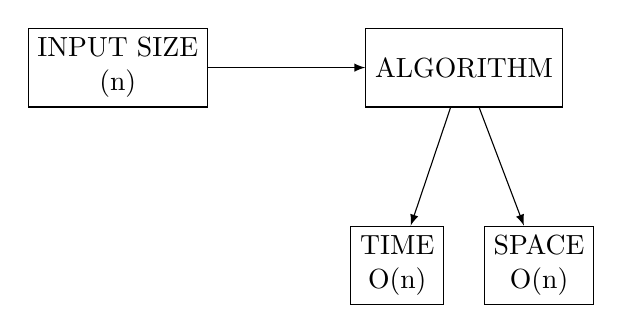
\begin{tikzpicture}[
    node distance=1.5cm,
    block/.style={rectangle, draw, minimum height=1cm, align=center},
    arrow/.style={-latex}
]
    \node[block] (input) {INPUT SIZE\\(n)};
    \node[block, right=2cm of input] (algo) {ALGORITHM};
    
    \node[block, below left=1.5cm and -1cm of algo] (time) {TIME\\O(n)};
    \node[block, below right=1.5cm and -1cm of algo] (space) {SPACE\\O(n)};
    
    \draw[arrow] (input) -- (algo);
    \draw[arrow] (algo) -- (time);
    \draw[arrow] (algo) -- (space);
\end{tikzpicture}
\captionof{figure}{Complexity Analysis}
\end{center}
\end{solutionbox}

\begin{mnemonicbox}
\mnemonic{Time Steps, Space Stores}
\end{mnemonicbox}

\questionmarks{1(c)}{7}{Explain concept of class \& object with example.}

\begin{solutionbox}
\begin{center}
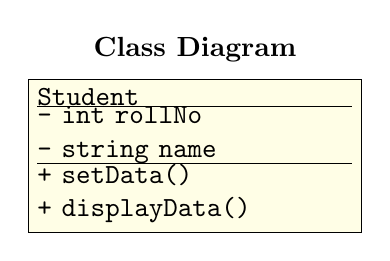
\begin{tikzpicture}[
    class/.style={rectangle, draw, fill=yellow!10, text width=4cm, align=left, font=\ttfamily},
    header/.style={fill=blue!20, align=center, font=\bfseries\sffamily}
]
    \node[class] (student) {
        \textbf{Student} \\ \hrule
        - int rollNo \\
        - string name \\ \hrule
        + setData() \\
        + displayData()
    };
    \node[above=0.1cm of student] {\textbf{Class Diagram}};
\end{tikzpicture}
\captionof{figure}{Student Class Structure}
\end{center}

\begin{center}
\captionof{table}{Class vs Object}
\begin{tabulary}{\linewidth}{|L|L|L|}
\hline
\textbf{Concept} & \textbf{Definition} & \textbf{Example} \\ \hline
Class & Blueprint or template for creating objects & Student class with properties (rollNo, name) and methods (setData, displayData) \\ \hline
Object & Instance of a class with specific values & student1 (rollNo=101, name="Raj") \\ \hline
\end{tabulary}
\end{center}

\textbf{Code Example:}
\begin{lstlisting}[language=Python]
class Student:
    def __init__(self):
        self.rollNo = 0
        self.name = ""
        
    def setData(self, r, n):
        self.rollNo = r
        self.name = n
        
    def displayData(self):
        print(self.rollNo, self.name)

# Creating objects
student1 = Student()
student1.setData(101, "Raj")
\end{lstlisting}
\end{solutionbox}

\begin{mnemonicbox}
\mnemonic{Class Creates, Objects Operate}
\end{mnemonicbox}

\questionmarks{1(c) OR}{7}{Develop a class for managing student records with instance methods for adding and removing students from a class.}

\begin{solutionbox}
\begin{center}
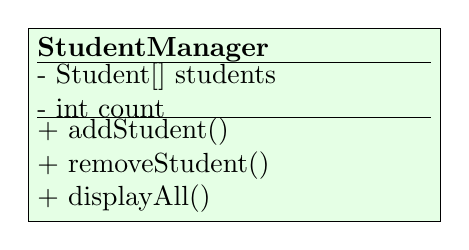
\begin{tikzpicture}[
    class/.style={rectangle, draw, fill=green!10, text width=5cm, align=left},
    header/.style={fill=green!30, align=center, font=\bfseries}
]
    \node[class] (manager) {
        \textbf{StudentManager} \\ \hrule
        - Student[] students \\
        - int count \\ \hrule
        + addStudent() \\
        + removeStudent() \\
        + displayAll()
    };
\end{tikzpicture}
\captionof{figure}{StudentManager Class}
\end{center}

\textbf{Code:}
\begin{lstlisting}[language=Python]
class StudentManager:
    def __init__(self):
        self.students = []
        
    def addStudent(self, roll, name):
        student = Student()
        student.setData(roll, name)
        self.students.append(student)
        
    def removeStudent(self, roll):
        for i in range(len(self.students)):
            if self.students[i].rollNo == roll:
                self.students.pop(i)
                break
    
    def displayAll(self):
        for student in self.students:
            student.displayData()
\end{lstlisting}
\end{solutionbox}

\begin{mnemonicbox}
\mnemonic{Add Accumulates, Remove Reduces}
\end{mnemonicbox}

\questionmarks{2(a)}{3}{Explain the importance of constructor in class.}

\begin{solutionbox}
\begin{center}
\captionof{table}{Constructor Importance}
\begin{tabulary}{\linewidth}{|L|}
\hline
\textbf{Constructor Importance} \\ \hline
1. Initializes object's data members \\ \hline
2. Automatically called when object is created \\ \hline
3. Can have different versions (default, parameterized, copy) \\ \hline
\end{tabulary}
\end{center}
\end{solutionbox}

\begin{mnemonicbox}
\mnemonic{Initialization Always Creates}
\end{mnemonicbox}

\questionmarks{2(b)}{4}{Explain different operations on stack.}

\begin{solutionbox}
\begin{center}
\captionof{table}{Stack Operations}
\begin{tabulary}{\linewidth}{|L|L|L|}
\hline
\textbf{Operation} & \textbf{Description} & \textbf{Example} \\ \hline
Push & Adds element to top & push(5) \\ \hline
Pop & Removes element from top & x = pop() \\ \hline
Peek/Top & Views top element without removing & x = peek() \\ \hline
isEmpty & Checks if stack is empty & if(isEmpty()) \\ \hline
\end{tabulary}
\end{center}

\begin{center}
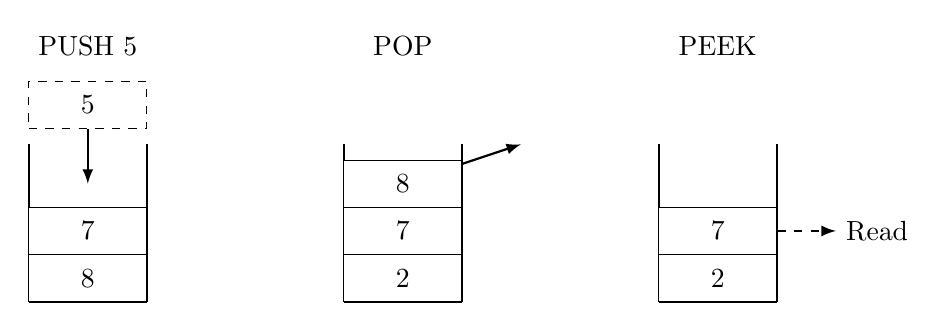
\begin{tikzpicture}[
    stack/.style={rectangle, draw, minimum width=1.5cm, minimum height=0.6cm, fill=white},
    arrow/.style={-latex, thick}
]
    % Push State
    \node[anchor=south] at (0, 3) {PUSH 5};
    \draw[thick] (-0.75, 0) -- (-0.75, 2) (0.75, 0) -- (0.75, 2) (-0.75, 0) -- (0.75, 0);
    \node[stack] at (0, 0.3) {8};
    \node[stack] at (0, 0.9) {7};
    \node[stack, dashed] (new) at (0, 2.5) {5};
    \draw[arrow] (new) -- (0, 1.5);

    % Pop State
    \begin{scope}[xshift=4cm]
    \node[anchor=south] at (0, 3) {POP};
    \draw[thick] (-0.75, 0) -- (-0.75, 2) (0.75, 0) -- (0.75, 2) (-0.75, 0) -- (0.75, 0);
    \node[stack] at (0, 0.3) {2};
    \node[stack] at (0, 0.9) {7};
    \node[stack] (top) at (0, 1.5) {8};
    \draw[arrow] (top) -- (1.5, 2);
    \end{scope}

    % Peek State
    \begin{scope}[xshift=8cm]
    \node[anchor=south] at (0, 3) {PEEK};
    \draw[thick] (-0.75, 0) -- (-0.75, 2) (0.75, 0) -- (0.75, 2) (-0.75, 0) -- (0.75, 0);
    \node[stack] at (0, 0.3) {2};
    \node[stack] (peek) at (0, 0.9) {7};
    \draw[arrow, dashed] (peek) -- (1.5, 0.9) node[right] {Read};
    \end{scope}
\end{tikzpicture}
\captionof{figure}{Stack Operations}
\end{center}
\end{solutionbox}

\begin{mnemonicbox}
\mnemonic{Push Pop Peek Properly}
\end{mnemonicbox}

\questionmarks{2(c)}{7}{Describe evaluation algorithm of postfix expression A B C + * D /}

\begin{solutionbox}
\begin{center}
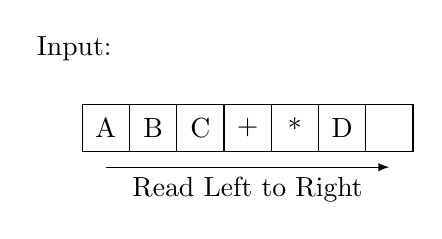
\begin{tikzpicture}[
    cell/.style={rectangle, draw, minimum size=0.6cm},
    arrow/.style={-latex}
]
    \node[anchor=west] at (-1, 1) {Input:};
    \foreach \x/\val in {0/A, 1/B, 2/C, 3/+, 4/*, 5/D, 6//} {
        \node[cell] at (\x*0.6, 0) {\val};
    }
    \draw[arrow] (0, -0.5) -- (3.6, -0.5) node[midway, below] {Read Left to Right};
\end{tikzpicture}
\captionof{figure}{Postfix Evaluation Process}
\end{center}

\begin{center}
\captionof{table}{Detailed Step-by-Step Trace}
\begin{tabulary}{\linewidth}{|C|C|L|L|}
\hline
\textbf{Step} & \textbf{Symbol} & \textbf{Action} & \textbf{Stack} \\ \hline
1 & A & Push onto stack & A \\ \hline
2 & B & Push onto stack & A, B \\ \hline
3 & C & Push onto stack & A, B, C \\ \hline
4 & + & Pop B, C; Push B+C & A, (B+C) \\ \hline
5 & * & Pop A, (B+C); Push A*(B+C) & A*(B+C) \\ \hline
6 & D & Push onto stack & A*(B+C), D \\ \hline
7 & / & Pop A*(B+C), D; Push result & (A*(B+C))/D \\ \hline
\end{tabulary}
\end{center}
\end{solutionbox}

\begin{mnemonicbox}
\mnemonic{Read, Push, Pop, Calculate}
\end{mnemonicbox}

\questionmarks{2(a) OR}{3}{Write difference between stack and queue.}

\begin{solutionbox}
\begin{center}
\captionof{table}{Stack vs Queue}
\begin{tabulary}{\linewidth}{|L|L|L|}
\hline
\textbf{Feature} & \textbf{Stack} & \textbf{Queue} \\ \hline
Principle & LIFO (Last In First Out) & FIFO (First In First Out) \\ \hline
Operations & Push/Pop & Enqueue/Dequeue \\ \hline
Access Points & Single end (top) & Two ends (front, rear) \\ \hline
\end{tabulary}
\end{center}
\end{solutionbox}

\begin{mnemonicbox}
\mnemonic{Stack LIFO, Queue FIFO}
\end{mnemonicbox}

\questionmarks{2(b) OR}{4}{Explain concept of circular queue.}

\begin{solutionbox}
\begin{center}
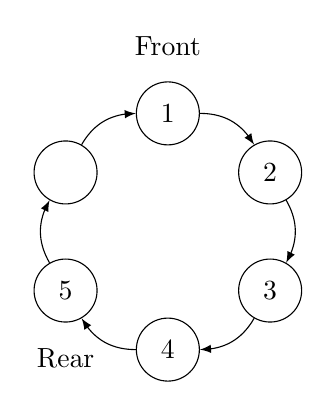
\begin{tikzpicture}[
    segment/.style={circle, draw, minimum size=0.8cm},
    arrow/.style={-latex}
]
    \node[segment] (n1) at (90:1.5) {1};
    \node[segment] (n2) at (30:1.5) {2};
    \node[segment] (n3) at (330:1.5) {3};
    \node[segment] (n4) at (270:1.5) {4};
    \node[segment] (n5) at (210:1.5) {5};
    \node[segment] (n6) at (150:1.5) {};

    \draw[arrow] (n1) to[bend left] (n2);
    \draw[arrow] (n2) to[bend left] (n3);
    \draw[arrow] (n3) to[bend left] (n4);
    \draw[arrow] (n4) to[bend left] (n5);
    \draw[arrow] (n5) to[bend left] (n6);
    \draw[arrow] (n6) to[bend left] (n1);

    \node[above=0.2cm of n1] {Front};
    \node[below=0.2cm of n5] {Rear};
\end{tikzpicture}
\captionof{figure}{Circular Queue Concept}
\end{center}

\begin{center}
\captionof{table}{Circular Queue Features}
\begin{tabulary}{\linewidth}{|L|L|}
\hline
\textbf{Feature} & \textbf{Description} \\ \hline
Structure & Linear data structure with connected ends \\ \hline
Advantage & Efficiently uses memory by reusing empty spaces \\ \hline
Operations & Enqueue, Dequeue with modulo arithmetic \\ \hline
\end{tabulary}
\end{center}
\end{solutionbox}

\begin{mnemonicbox}
\mnemonic{Circular Connects Front to Rear}
\end{mnemonicbox}

\questionmarks{2(c) OR}{7}{Describe the procedure for inserting a new node after and before a given node in a singly linked list.}

\begin{solutionbox}
\begin{center}
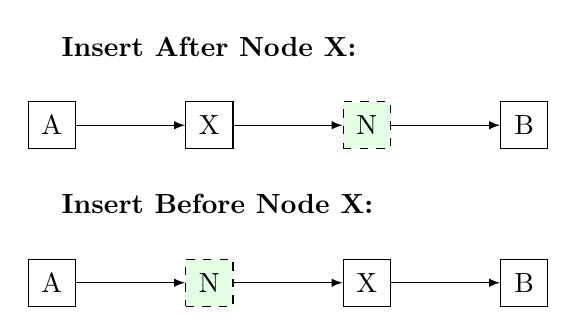
\begin{tikzpicture}[
    listnode/.style={rectangle, draw, minimum size=0.6cm},
    arrow/.style={-latex}
]
    % Insert After
    \node[anchor=west] at (0, 3) {\textbf{Insert After Node X:}};
    \node[listnode] (a) at (0, 2) {A};
    \node[listnode] (x) at (2, 2) {X};
    \node[listnode, dashed, fill=green!10] (n) at (4, 2) {N};
    \node[listnode] (b) at (6, 2) {B};
    
    \draw[arrow] (a) -- (x);
    \draw[arrow] (x) -- (n);
    \draw[arrow] (n) -- (b);

    % Insert Before
    \node[anchor=west] at (0, 1) {\textbf{Insert Before Node X:}};
    \node[listnode] (a2) at (0, 0) {A};
    \node[listnode, dashed, fill=green!10] (n2) at (2, 0) {N};
    \node[listnode] (x2) at (4, 0) {X};
    \node[listnode] (b2) at (6, 0) {B};

    \draw[arrow] (a2) -- (n2);
    \draw[arrow] (n2) -- (x2);
    \draw[arrow] (x2) -- (b2);
\end{tikzpicture}
\captionof{figure}{Insertion in Singly Linked List}
\end{center}

\begin{center}
\captionof{table}{Insertion Procedure}
\begin{tabulary}{\linewidth}{|L|L|}
\hline
\textbf{Insertion} & \textbf{Steps} \\ \hline
After Node X & 1. Create new node N \newline 2. Set N's next to X's next \newline 3. Set X's next to N \\ \hline
Before Node X & 1. Create new node N \newline 2. Find node A pointing to X \newline 3. Set N's next to X \newline 4. Set A's next to N \\ \hline
\end{tabulary}
\end{center}
\end{solutionbox}

\questionmarks{3(a)}{3}{Explain traversing a linked list.}

\begin{solutionbox}
\begin{center}
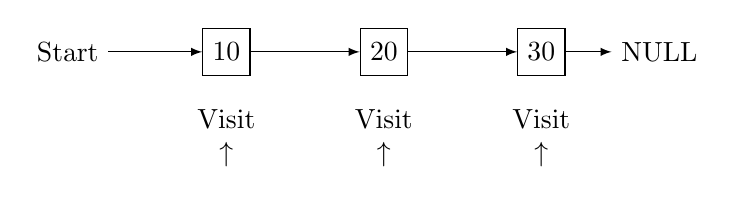
\begin{tikzpicture}[
    listnode/.style={rectangle, draw, minimum size=0.6cm},
    arrow/.style={-latex}
]
    \node[anchor=east] (start) at (0, 0) {Start};
    \node[listnode] (n1) at (1.5, 0) {10};
    \node[listnode] (n2) at (3.5, 0) {20};
    \node[listnode] (n3) at (5.5, 0) {30};
    \node (null) at (7, 0) {NULL};

    \draw[arrow] (start) -- (n1);
    \draw[arrow] (n1) -- (n2);
    \draw[arrow] (n2) -- (n3);
    \draw[arrow] (n3) -- (null);

    \node[below=0.3cm of n1, align=center] {Visit\\$\uparrow$};
    \node[below=0.3cm of n2, align=center] {Visit\\$\uparrow$};
    \node[below=0.3cm of n3, align=center] {Visit\\$\uparrow$};
\end{tikzpicture}
\captionof{figure}{Linked List Traversal}
\end{center}

\begin{center}
\captionof{table}{Traversal Steps}
\begin{tabulary}{\linewidth}{|C|L|}
\hline
\textbf{Step} & \textbf{Action} \\ \hline
1 & Initialize pointer to head \\ \hline
2 & Access data at current node \\ \hline
3 & Move pointer to next node \\ \hline
4 & Repeat until NULL \\ \hline
\end{tabulary}
\end{center}
\end{solutionbox}

\begin{mnemonicbox}
\mnemonic{Start, Access, Move, Repeat}
\end{mnemonicbox}

\questionmarks{3(b)}{4}{Explain expression conversion from infix to postfix.}

\begin{solutionbox}
\begin{center}
\begin{tcolorbox}[colback=blue!5, colframe=blue!40, title=Example Conversion]
\textbf{Infix:} $A + B * C$ \\
\textbf{Postfix:} $A \ B \ C \ * \ +$
\end{tcolorbox}
\end{center}

\begin{center}
\captionof{table}{Conversion Algorithm Trace}
\begin{tabulary}{\linewidth}{|C|L|C|L|}
\hline
\textbf{Step} & \textbf{Action} & \textbf{Stack} & \textbf{Output} \\ \hline
1 & Scan from left to right & & \\ \hline
2 & If operand, add to output & & A \\ \hline
3 & If operator, push if higher precedence & + & A \\ \hline
4 & Pop lower precedence operators & + & A B \\ \hline
5 & Push current operator & * & A B \\ \hline
6 & Continue until expression ends & * & A B C \\ \hline
7 & Pop remaining operators & & A B C * + \\ \hline
\end{tabulary}
\end{center}
\end{solutionbox}

\begin{mnemonicbox}
\mnemonic{Operators Push Pop, Operands Output Directly}
\end{mnemonicbox}

\questionmarks{3(c)}{7}{Write a program to delete a node at the beginning and end of singly linked list.}

\begin{solutionbox}
\begin{center}
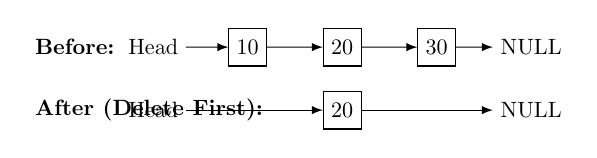
\begin{tikzpicture}[
    listnode/.style={rectangle, draw, minimum size=0.6cm},
    arrow/.style={-latex},
    scale=0.8, transform shape
]
    \node[anchor=west] at (-2, 1) {\textbf{Before:}};
    \node (head) at (0, 1) {Head};
    \node[listnode] (n1) at (1.5, 1) {10};
    \node[listnode] (n2) at (3, 1) {20};
    \node[listnode] (n3) at (4.5, 1) {30};
    \node (null) at (6, 1) {NULL};
    \draw[arrow] (head) -- (n1); \draw[arrow] (n1) -- (n2); \draw[arrow] (n2) -- (n3); \draw[arrow] (n3) -- (null);

    \node[anchor=west] at (-2, 0) {\textbf{After (Delete First):}};
    \node (head2) at (0, 0) {Head};
    \node[listnode] (n22) at (3, 0) {20};
    \node (null2) at (6, 0) {NULL};
    \draw[arrow] (head2) -- (n22); \draw[arrow] (n22) -- (null2);
\end{tikzpicture}
\captionof{figure}{Deletion Visualization}
\end{center}

\textbf{Code:}
\begin{lstlisting}[language=Python]
class Node:
    def __init__(self, data):
        self.data = data
        self.next = None

class LinkedList:
    def __init__(self):
        self.head = None
    
    def deleteFirst(self):
        if self.head is None:
            return
        self.head = self.head.next
    
    def deleteLast(self):
        if self.head is None:
            return
        
        # If only one node
        if self.head.next is None:
            self.head = None
            return
            
        temp = self.head
        while temp.next.next:
            temp = temp.next
        
        temp.next = None
\end{lstlisting}
\end{solutionbox}

\begin{mnemonicbox}
\mnemonic{Delete First: Shift Head, Delete Last: Find Second-Last}
\end{mnemonicbox}

\questionmarks{3(a) OR}{3}{Explain searching an element in linked list.}

\begin{solutionbox}
\begin{center}
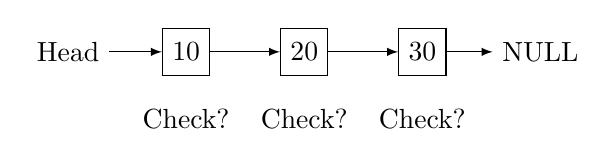
\begin{tikzpicture}[
    listnode/.style={rectangle, draw, minimum size=0.6cm},
    arrow/.style={-latex}
]
    \node (head) at (0, 0) {Head};
    \node[listnode] (n1) at (1.5, 0) {10};
    \node[listnode] (n2) at (3, 0) {20};
    \node[listnode] (n3) at (4.5, 0) {30};
    \node (null) at (6, 0) {NULL};

    \draw[arrow] (head) -- (n1); \draw[arrow] (n1) -- (n2); \draw[arrow] (n2) -- (n3); \draw[arrow] (n3) -- (null);
    
    \node[below=0.3cm of n1] {Check?};
    \node[below=0.3cm of n2] {Check?};
    \node[below=0.3cm of n3] {Check?};
\end{tikzpicture}
\captionof{figure}{Linear Search in Linked List}
\end{center}

\begin{center}
\captionof{table}{Search Steps}
\begin{tabulary}{\linewidth}{|C|L|}
\hline
\textbf{Step} & \textbf{Description} \\ \hline
1 & Start from head node \\ \hline
2 & Compare current node's data with key \\ \hline
3 & If match found, return true \\ \hline
4 & Else, move to next node and repeat \\ \hline
\end{tabulary}
\end{center}
\end{solutionbox}

\begin{mnemonicbox}
\mnemonic{Start, Compare, Move, Repeat}
\end{mnemonicbox}

\questionmarks{3(b) OR}{4}{Explain concepts of circular linked lists.}

\begin{solutionbox}
\begin{center}
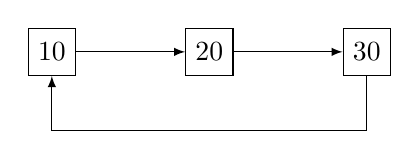
\begin{tikzpicture}[
    listnode/.style={rectangle, draw, minimum size=0.6cm},
    arrow/.style={-latex}
]
    \node[listnode] (n1) at (0, 0) {10};
    \node[listnode] (n2) at (2, 0) {20};
    \node[listnode] (n3) at (4, 0) {30};

    \draw[arrow] (n1) -- (n2);
    \draw[arrow] (n2) -- (n3);
    \draw[arrow] (n3) -- (4, -1) -- (0, -1) -- (n1);
\end{tikzpicture}
\captionof{figure}{Circular Linked List}
\end{center}

\begin{center}
\captionof{table}{Circular LL Features}
\begin{tabulary}{\linewidth}{|L|L|}
\hline
\textbf{Feature} & \textbf{Description} \\ \hline
Structure & Last node points to first node \\ \hline
Advantage & No NULL pointers, efficient for circular operations \\ \hline
Traversal & Need extra condition to prevent infinite loop \\ \hline
\end{tabulary}
\end{center}
\end{solutionbox}

\begin{mnemonicbox}
\mnemonic{Last Links to First}
\end{mnemonicbox}

\questionmarks{3(c) OR}{7}{Explain algorithm to search a particular element from list using Binary Search.}

\begin{solutionbox}
\begin{center}
\begin{tikzpicture}[node distance=1.5cm]
    \node[gtu block] (start) {Start};
    \node[gtu block, right=of start] (init) {Low=0, High=n-1};
    \node[gtu decision, right=of init] (check) {Low $\le$ High?};
    \node[gtu block, below=of check] (mid) {Mid = (L+H)/2};
    \node[gtu decision, below=of mid] (compare) {A[Mid] == Key?};
    \node[gtu state, right=of compare] (found) {Return Mid};
    
    \node[gtu decision, left=of compare] (smaller) {A[Mid] < Key?};
    \node[gtu block, above=of smaller] (right) {Low = Mid+1};
    \node[gtu block, left=of smaller] (left) {High = Mid-1};
    \node[gtu state, right=of check] (notfound) {Return -1};

    \path[gtu arrow] (start) -- (init);
    \path[gtu arrow] (init) -- (check);
    \path[gtu arrow] (check) -- node[right] {Yes} (mid);
    \path[gtu arrow] (check) -- node[above] {No} (notfound);
    \path[gtu arrow] (mid) -- (compare);
    \path[gtu arrow] (compare) -- node[above] {Yes} (found);
    \path[gtu arrow] (compare) -- node[above] {No} (smaller);
    \path[gtu arrow] (smaller) -- node[left] {Yes} (right);
    \path[gtu arrow] (smaller) -- node[above] {No} (left);
    \path[gtu arrow] (right) |- (check);
    \path[gtu arrow] (left) |- (check);

\end{tikzpicture}
\captionof{figure}{Binary Search Flowchart}
\end{center}

\textbf{Code:}
\begin{lstlisting}[language=Python]
def binarySearch(arr, key):
    low = 0
    high = len(arr) - 1
    
    while low <= high:
        mid = (low + high) // 2
        
        if arr[mid] == key:
            return mid
        elif arr[mid] < key:
            low = mid + 1
        else:
            high = mid - 1
            
    return -1
\end{lstlisting}
\end{solutionbox}

\begin{mnemonicbox}
\mnemonic{Middle, Compare, Eliminate Half}
\end{mnemonicbox}

\questionmarks{4(a)}{3}{Write applications of linked list.}

\begin{solutionbox}
\begin{center}
\captionof{table}{Applications of Linked List}
\begin{tabulary}{\linewidth}{|L|}
\hline
\textbf{Applications} \\ \hline
1. Implementation of stacks and queues \\ \hline
2. Dynamic memory allocation \\ \hline
3. Image viewer (next/previous images) \\ \hline
\end{tabulary}
\end{center}
\end{solutionbox}

\begin{mnemonicbox}
\mnemonic{Store Data Dynamically}
\end{mnemonicbox}

\questionmarks{4(b)}{4}{Differentiate between singly linked list and doubly linked list.}

\begin{solutionbox}
\begin{center}
\captionof{table}{Singly vs Doubly Linked List}
\begin{tabulary}{\linewidth}{|L|L|L|}
\hline
\textbf{Feature} & \textbf{Singly Linked List} & \textbf{Doubly Linked List} \\ \hline
Node Structure & One pointer (next) & Two pointers (next, prev) \\ \hline
Traversal & Forward only & Both directions \\ \hline
Memory & Less memory & More memory \\ \hline
Operations & Simple, less code & Complex, more flexible \\ \hline
\end{tabulary}
\end{center}

\begin{center}
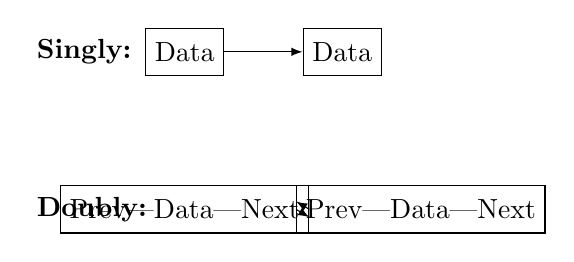
\begin{tikzpicture}[
    listnode/.style={rectangle, draw, minimum size=0.6cm},
    dnode/.style={rectangle, draw, minimum width=1.8cm, minimum height=0.6cm},
    arrow/.style={-latex}
]
    \node[anchor=west] at (0, 2) {\textbf{Singly:}};
    \node[listnode] (s1) at (2, 2) {Data}; \node[listnode] (s2) at (4, 2) {Data};
    \draw[arrow] (s1) -- (s2);

    \node[anchor=west] at (0, 0) {\textbf{Doubly:}};
    \node[dnode] (d1) at (2, 0) {Prev|Data|Next};
    \node[dnode] (d2) at (5, 0) {Prev|Data|Next};
    
    \draw[arrow] (d1.east) -- ([yshift=0.1cm]d2.west);
    \draw[arrow] (d2.west) -- ([yshift=-0.1cm]d1.east);
\end{tikzpicture}
\captionof{figure}{Node Structures}
\end{center}
\end{solutionbox}

\begin{mnemonicbox}
\mnemonic{Single Direction, Double Direction}
\end{mnemonicbox}

\questionmarks{4(c)}{7}{Write a program to sort numbers in ascending order using selection sort algorithm.}

\begin{solutionbox}
\begin{center}
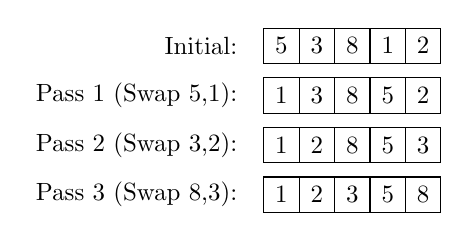
\begin{tikzpicture}[
    cell/.style={rectangle, draw, minimum size=0.5cm},
    scale=0.9, transform shape
]
    \foreach \x/\val in {0/5, 1/3, 2/8, 3/1, 4/2} \node[cell] at (\x*0.5, 0) {\val};
    \node[anchor=east] at (-0.5, 0) {Initial:};

    \foreach \x/\val in {0/1, 1/3, 2/8, 3/5, 4/2} \node[cell] at (\x*0.5, -0.7) {\val};
    \node[anchor=east] at (-0.5, -0.7) {Pass 1 (Swap 5,1):};

    \foreach \x/\val in {0/1, 1/2, 2/8, 3/5, 4/3} \node[cell] at (\x*0.5, -1.4) {\val};
    \node[anchor=east] at (-0.5, -1.4) {Pass 2 (Swap 3,2):};

    \foreach \x/\val in {0/1, 1/2, 2/3, 3/5, 4/8} \node[cell] at (\x*0.5, -2.1) {\val};
    \node[anchor=east] at (-0.5, -2.1) {Pass 3 (Swap 8,3):};
\end{tikzpicture}
\captionof{figure}{Selection Sort Calculation}
\end{center}

\textbf{Code:}
\begin{lstlisting}[language=Python]
def selectionSort(arr):
    n = len(arr)
    
    for i in range(n):
        min_idx = i
        
        for j in range(i+1, n):
            if arr[j] < arr[min_idx]:
                min_idx = j
        
        # Swap the found minimum element with the first element
        arr[i], arr[min_idx] = arr[min_idx], arr[i]
    
    return arr

# Example usage
arr = [5, 3, 8, 1, 2]
sorted_arr = selectionSort(arr)
print(sorted_arr)  # Output: [1, 2, 3, 5, 8]
\end{lstlisting}
\end{solutionbox}

\begin{mnemonicbox}
\mnemonic{Find Minimum, Swap Position}
\end{mnemonicbox}

\questionmarks{4(a) OR}{3}{Explain bubble sort algorithm.}

\begin{solutionbox}
\begin{center}
\begin{tikzpicture}[node distance=1.2cm]
    \node[gtu block] (p1) {Pass 1};
    \node[gtu block, right=of p1] (p2) {Pass 2};
    \node[gtu block, right=of p2] (p3) {Pass 3};
    \node[gtu state, right=of p3] (sorted) {Sorted};

    \draw[gtu arrow] (p1) -- (p2);
    \draw[gtu arrow] (p2) -- (p3);
    \draw[gtu arrow] (p3) -- (sorted);
\end{tikzpicture}
\captionof{figure}{Bubble Sort Flow}
\end{center}

\begin{center}
\captionof{table}{Key Points}
\begin{tabulary}{\linewidth}{|L|}
\hline
\textbf{Key Points} \\ \hline
Compare adjacent elements \\ \hline
Swap if they are in wrong order \\ \hline
Largest element bubbles to end in each pass \\ \hline
\end{tabulary}
\end{center}
\end{solutionbox}

\begin{mnemonicbox}
\mnemonic{Bubble Bigger Elements Upward}
\end{mnemonicbox}

\questionmarks{4(b) OR}{4}{Differentiate Linear \& Binary search.}

\begin{solutionbox}
\begin{center}
\captionof{table}{Linear vs Binary Search}
\begin{tabulary}{\linewidth}{|L|L|L|}
\hline
\textbf{Feature} & \textbf{Linear Search} & \textbf{Binary Search} \\ \hline
Working Principle & Sequential checking & Divide and conquer \\ \hline
Time Complexity & O(n) & O(log n) \\ \hline
Data Arrangement & Unsorted or sorted & Must be sorted \\ \hline
Best For & Small datasets & Large datasets \\ \hline
\end{tabulary}
\end{center}
\end{solutionbox}

\begin{mnemonicbox}
\mnemonic{Linear Looks at All, Binary Breaks in Half}
\end{mnemonicbox}

\questionmarks{4(c) OR}{7}{Explain Quick sort \& Merge sort algorithm.}

\begin{solutionbox}
\textbf{Quick Sort:}
\begin{center}
\begin{tikzpicture}[node distance=1.2cm]
    \node[gtu block] (start) {Quick Sort};
    \node[gtu block, right=of start] (pivot) {Select Pivot};
    \node[gtu block, right=of pivot] (part) {Partition};
    \node[gtu block, above right=of part] (left) {Sort Left};
    \node[gtu block, below right=of part] (right) {Sort Right};

    \draw[gtu arrow] (start) -- (pivot);
    \draw[gtu arrow] (pivot) -- (part);
    \draw[gtu arrow] (part) -- (left);
    \draw[gtu arrow] (part) -- (right);
\end{tikzpicture}
\end{center}

\textbf{Merge Sort:}
\begin{center}
\begin{tikzpicture}[node distance=1.2cm]
    \node[gtu block] (start) {Merge Sort};
    \node[gtu block, right=of start] (divide) {Divide Half};
    \node[gtu block, above right=of divide] (left) {Sort Left};
    \node[gtu block, below right=of divide] (right) {Sort Right};
    \node[gtu state, right=of divide, xshift=2cm] (merge) {Merge};

    \draw[gtu arrow] (start) -- (divide);
    \draw[gtu arrow] (divide) -- (left);
    \draw[gtu arrow] (divide) -- (right);
    \draw[gtu arrow] (left) -- (merge);
    \draw[gtu arrow] (right) -- (merge);
\end{tikzpicture}
\end{center}

\begin{center}
\captionof{table}{Complexity Comparison}
\begin{tabulary}{\linewidth}{|L|L|L|L|}
\hline
\textbf{Algorithm} & \textbf{Principle} & \textbf{Avg Time} & \textbf{Space} \\ \hline
Quick Sort & Partitioning around pivot & O(n log n) & O(log n) \\ \hline
Merge Sort & Divide, conquer, combine & O(n log n) & O(n) \\ \hline
\end{tabulary}
\end{center}
\end{solutionbox}

\questionmarks{5(a)}{3}{Define a complete binary tree.}

\begin{solutionbox}
\begin{center}
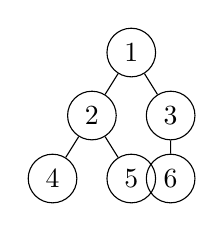
\begin{tikzpicture}[
    treenode/.style={circle, draw, minimum size=0.6cm},
    level distance=0.8cm,
    sibling distance=1cm
]
    \node[treenode] {1}
        child {node[treenode] {2}
            child {node[treenode] {4}}
            child {node[treenode] {5}}
        }
        child {node[treenode] {3}
            child {node[treenode] {6}}
        };
\end{tikzpicture}
\captionof{figure}{Complete Binary Tree}
\end{center}

\begin{center}
\captionof{table}{Properties}
\begin{tabulary}{\linewidth}{|L|L|}
\hline
\textbf{Property} & \textbf{Description} \\ \hline
All levels filled & Except possibly the last level \\ \hline
Last level filled from left & Nodes added from left to right \\ \hline
\end{tabulary}
\end{center}
\end{solutionbox}

\begin{mnemonicbox}
\mnemonic{Fill Left to Right, Level by Level}
\end{mnemonicbox}

\questionmarks{5(b)}{4}{Explain inorder traversal of a binary tree.}

\begin{solutionbox}
\begin{center}
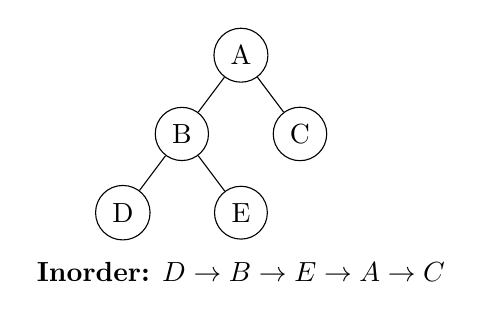
\begin{tikzpicture}[
    treenode/.style={circle, draw, minimum size=0.6cm},
    level distance=1cm,
    sibling distance=1.5cm
]
    \node[treenode] {A}
        child {node[treenode] {B}
            child {node[treenode] {D}}
            child {node[treenode] {E}}
        }
        child {node[treenode] {C}};
    
    \node[below=2.5cm] {\textbf{Inorder:} $D \rightarrow B \rightarrow E \rightarrow A \rightarrow C$};
\end{tikzpicture}
\captionof{figure}{Inorder Traversal}
\end{center}

\begin{center}
\captionof{table}{Algorithm Steps}
\begin{tabulary}{\linewidth}{|C|L|}
\hline
\textbf{Step} & \textbf{Action} \\ \hline
1 & Traverse left subtree \\ \hline
2 & Visit root node \\ \hline
3 & Traverse right subtree \\ \hline
\end{tabulary}
\end{center}

\textbf{Code:}
\begin{lstlisting}[language=Python]
def inorderTraversal(root):
    if root:
        inorderTraversal(root.left)
        print(root.data, end=" -> ")
        inorderTraversal(root.right)
\end{lstlisting}
\end{solutionbox}

\begin{mnemonicbox}
\mnemonic{Left, Root, Right}
\end{mnemonicbox}

\questionmarks{5(c)}{7}{Write a program to inserting a node into a binary search tree.}

\begin{solutionbox}
\begin{center}
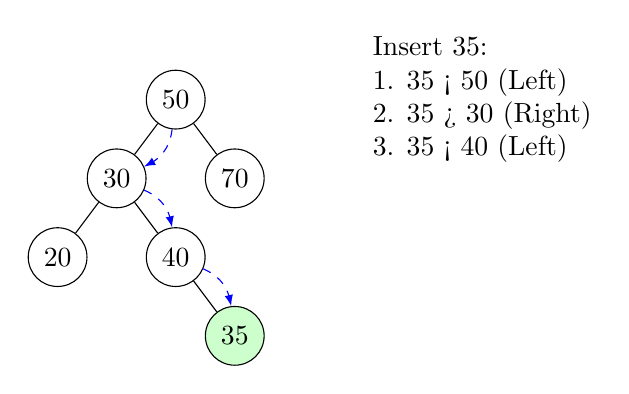
\begin{tikzpicture}[
    treenode/.style={circle, draw, minimum size=0.6cm},
    level distance=1cm,
    sibling distance=1.5cm,
    arrow/.style={-latex, dashed, blue}
]
    \node[treenode] (50) {50}
        child {node[treenode] (30) {30}
            child {node[treenode] (20) {20}}
            child {node[treenode] (40) {40}
                child[missing] {}
                child {node[treenode, fill=green!20] (35) {35}}
            }
        }
        child {node[treenode] (70) {70}};
        
    \draw[arrow] (50) to[bend left] (30);
    \draw[arrow] (30) to[bend left] (40);
    \draw[arrow] (40) to[bend left] (35);
    
    \node[right=2cm of 50, align=left] {Insert 35:\\1. 35 < 50 (Left)\\2. 35 > 30 (Right)\\3. 35 < 40 (Left)};
\end{tikzpicture}
\captionof{figure}{Insertion Process}
\end{center}

\textbf{Code:}
\begin{lstlisting}[language=Python]
class Node:
    def __init__(self, key):
        self.key = key
        self.left = None
        self.right = None

def insert(root, key):
    if root is None:
        return Node(key)
    
    if key < root.key:
        root.left = insert(root.left, key)
    else:
        root.right = insert(root.right, key)
        
    return root
\end{lstlisting}
\end{solutionbox}

\begin{mnemonicbox}
\mnemonic{Compare, Move, Insert}
\end{mnemonicbox}

\questionmarks{5(a) OR}{3}{State the fundamental characteristic of a binary search tree.}

\begin{solutionbox}
\begin{center}
\captionof{table}{BST Characteristics}
\begin{tabulary}{\linewidth}{|L|}
\hline
\textbf{Characteristics} \\ \hline
1. Left child nodes < Parent node \\ \hline
2. Right child nodes > Parent node \\ \hline
3. No duplicate values allowed \\ \hline
\end{tabulary}
\end{center}
\end{solutionbox}

\begin{mnemonicbox}
\mnemonic{Left Less, Right More}
\end{mnemonicbox}

\questionmarks{5(b) OR}{4}{Explain postorder traversal of a binary tree.}

\begin{solutionbox}
\begin{center}
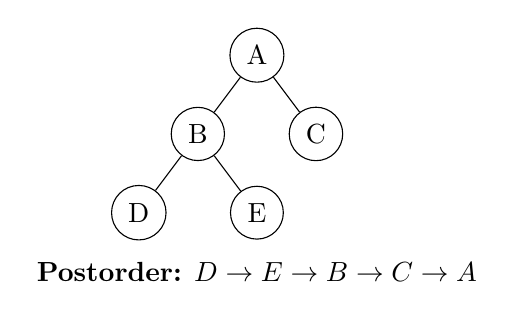
\begin{tikzpicture}[
    treenode/.style={circle, draw, minimum size=0.6cm},
    level distance=1cm,
    sibling distance=1.5cm
]
    \node[treenode] {A}
        child {node[treenode] {B}
            child {node[treenode] {D}}
            child {node[treenode] {E}}
        }
        child {node[treenode] {C}};
    
    \node[below=2.5cm] {\textbf{Postorder:} $D \rightarrow E \rightarrow B \rightarrow C \rightarrow A$};
\end{tikzpicture}
\captionof{figure}{Postorder Traversal}
\end{center}

\begin{center}
\captionof{table}{Step-by-Step}
\begin{tabulary}{\linewidth}{|C|L|}
\hline
\textbf{Step} & \textbf{Action} \\ \hline
1 & Traverse left subtree \\ \hline
2 & Traverse right subtree \\ \hline
3 & Visit root node \\ \hline
\end{tabulary}
\end{center}

\textbf{Code:}
\begin{lstlisting}[language=Python]
def postorderTraversal(root):
    if root:
        postorderTraversal(root.left)
        postorderTraversal(root.right)
        print(root.data, end=" -> ")
\end{lstlisting}
\end{solutionbox}

\begin{mnemonicbox}
\mnemonic{Left, Right, Root}
\end{mnemonicbox}

\questionmarks{5(c) OR}{7}{Write a program to delete a node from a binary search tree.}

\begin{solutionbox}
\begin{center}
\begin{tikzpicture}[node distance=1.5cm]
    \node[gtu block] (start) {Find Node};
    \node[gtu decision, below=of start] (zero) {0 Children?};
    \node[gtu state, right=of zero] (rem) {Remove};
    \node[gtu decision, below=of zero] (one) {1 Child?};
    \node[gtu state, right=of one] (repl) {Replace w/ Child};
    \node[gtu state, below=of one] (succ) {Replace w/ Successor};

    \draw[gtu arrow] (start) -- (zero);
    \draw[gtu arrow] (zero) -- node[above] {Yes} (rem);
    \draw[gtu arrow] (zero) -- node[right] {No} (one);
    \draw[gtu arrow] (one) -- node[above] {Yes} (repl);
    \draw[gtu arrow] (one) -- node[right] {No} (succ);
\end{tikzpicture}
\captionof{figure}{Deletion Logic}
\end{center}

\textbf{Code:}
\begin{lstlisting}[language=Python]
def minValueNode(node):
    current = node
    while current.left is not None:
        current = current.left
    return current

def deleteNode(root, key):
    if root is None: return root

    if key < root.key:
        root.left = deleteNode(root.left, key)
    elif key > root.key:
        root.right = deleteNode(root.right, key)
    else:
        # Node with only one child or no child
        if root.left is None:
            return root.right
        elif root.right is None:
            return root.left

        # Node with two children
        temp = minValueNode(root.right)
        root.key = temp.key
        root.right = deleteNode(root.right, temp.key)

    return root
\end{lstlisting}
\end{solutionbox}

\begin{mnemonicbox}
\mnemonic{Zero: Remove, One: Replace, Two: Successor}
\end{mnemonicbox}

\end{document}


